%% grundlagen.tex
%% $Id: grundlagen.tex 28 2007-01-18 16:31:32Z bless $
%%

\chapter{Grundlagen}
\label{ch:Grundlagen}
%% ==============================
Die Grundlagen müssen soweit beschrieben
werden, dass ein Leser das Problem und
die Probleml{\"o}sung  versteht.Um nicht zuviel 
zu beschreiben, kann man das auch erst gegen 
Ende der Arbeit schreiben.

Bla fasel\ldots

%% ==============================
\section{Tactile Ger{\"a}te}
%% ==============================
\label{ch:Grundlagen:sec:Taktile Ger{\"a}te}

Bla fasel\ldots

%% taktile ger{\"a}ate.tex
%% $Id: taktilegeraete.tex 28 2007-01-18 16:31:32Z bless $
%%

Ein Taktiles Ger{\"a}t ist ein Ger{\"a}t, dass Informationen an einen Menschen durch die Wahrnehmung der Haut mitteilt.\cite{gemperle2001design}
% mitteilen m{\"o}chte, dies geschieht durch die Wahrnehmung der Haut. 

Taktile Ger{\"a}te werden heutzutage {\"o}fter verwendet, als man es eigentlich wahrnimmt. 
Ein einfaches Beispiel ist das Smartphone. 
Eine Person trägt sein eigenes Smartphone in der Hosentasche. 
Bei einer eingehenden Nachricht, muss der Benutzer mitgeteilt werden, dass eine Nachricht empfangen wurde.
Normalerweise geschieht das beim Abspielen des Klingeltons. Falls man besch{\"a}ftigt ist und nicht durch ein lautes Klingeln gest{\"o}rt werden will, stellt man den Ton ab. 
Um dennoch den Nutzer darauf Aufmerksam zu machen, dass eine Nachricht eingetroffen ist, wird die Vibration des Smartphones verwendet.
%spielt die Vibration des Smartphones eine große Rolle. 
%verwendet man die Vibration des Smartphones.
%Um dennoch darauf Aufmerksam zu machen, dass eine Nachricht eingetroffen ist, nutzt man die Vibration des Smartphones.

%Das Smartphone ist nur eins von vielen Beispielen, was man {\"u}ber den Alltag noch f{\"u}r Taktile Ger{\"a}te verwendet.
Ein weiteres Beispiel in der Taktile Displays benutzt werden ist f{\"u}r Blinde Menschen, um Wissen zu {\"u}bermitteln \cite{parente2003bats}. 
F{\"u}r Blinde gibt es spezielle Karten, die Konturen f{\"u}r die Umrisse der L{\"a}nder darstellen, solche Karten sind selten vertreten.
Um ein solches Ungleichgewicht zwischen den blinden und normal sehenden Sch{\"u}lern zu mindern, hat man sich ein System entwickelt, dass audiovisuelle und taktile Eindr{\"u}cke vereint. 
Dabei hat man sich f{\"u}r eines r{\"a}umlich akustisches Soundsystem entschieden, um den Sch{\"u}ler anhand Ger{\"a}uschen aus verschiedenen Richtungen ein Gef{\"u}hl zu geben, an welchen Orten man sich aktuell befindet und was um einen herum passiert. 
Es wurden nicht nur Tier- und Verkehrsger{\"a}usche verwendet, sondern auch den Namen der Region, in der man sich aktuell befindet, wurde ausgespeochen. 
Als Taktiles Device hat man sich an schon existierenden M{\"a}usen und Controllern bedient, die Force-Feedback besa{\ss}en. 

Die verwendeten Karten waren nicht so detailliert wie in der Realit{\"a}t.
%Die Karten, die man verwendet hat, sind nicht so detailliert, wie normale Karten. 
Im Vergleich zu der normalen Karten hat man hier weniger Informationen, die man {\"u}bertragen muss und die Details der L{\"a}ndergrenzen konnte man leichter darstellen. 

Damit ein Sch{\"u}ler eine Karte erkunden konnte, bewegt er sich mithilfe eines Eingabeger{\"a}ts {\"u}ber die Karte und dr{\"u}ckt eine Taste auf der Tastatur um Informationen {\"u}ber das Gebiet abzurufen, diese wurden {\"u}ber Audios {\"u}bermittelt. Das Taktile Device wurde verwendet um Grenz{\"u}berg{\"a}nge zu mittels Vibrationen zu signalisieren.





%% ==============================
\section{Genetischer Algorithmus}
%% ==============================
\label{ch:Grundlagen:sec:Genetischer Algorithmus}

Bla fasel\ldots
%% Genetischer Algorithmus.tex
%% $Id: Genetischer Algorithmus.tex 28 2007-01-18 16:31:32Z bless $
%%

Die Evalutionären Algorithmen sind stochastische Optimierungsverfahren. Man findet damit nicht die beste Lösung für ein Problem, jedoch findet man eine gute Annäherung.
Dabei hat man sich bei den Evolutionären Algorithmen an der Biologischen Evolution von Darwin inspirieren lassen. \cite{selzam2003genetische}

In der Biologie ist jeder lebende Organismus ein Induvidiuum.
Jedes Induvidiuum besitzt Erbinformationen in der Form von Chromosomen. Die Erbinformationen werden auch \textbf{Gene} oder \textbf{DNA} genannt.
Eine Gruppe von Induviduen wird als \textbf{Population} bezeichnet.

Der Algorithmus wurde anhand der folgenden Merkmale erstellt.

%% ==============================
\subsection{Selektion}
%% ==============================
\label{ch:Grundlagen:sec:Taktile Geräte:subsec:Selektion}

Eine \textbf{Selektion} ist ein Mechanismus, bei dem man sich zwei Individuen auswählt, um anschließend die Gene der beiden Individuen, mittels der sogenannten \textbf{Rekombination}, zu kombinieren. Dabei gibt es verschiedene Selektionsstrategien. Man versucht die Individuen zu finden, um eine bestmöglichste Lösung für ein Problem zu liefern.

%% ==============================
\subsection{Variation}
%% ==============================
\label{ch:Grundlagen:sec:Taktile Geräte:subsec:Variation}

Man sollte eine zahlreiche Variation von Genen der einzelnen Individuen besitzen. 
Denn nehme anhand einem Beispiel von Süßigkeiten einmal kurz an, dass alle Süßigkeiten die gleiche Farbe und die gleiche Form haben. Wenn man sich jetzt zwei zufällige Süßigkeiten auswählen würde, hätten Sie keinerlei unterschiede und so würde das Nachkommen die gleichen Gene besitzen. Damit genau das nicht auftaucht, versucht man zu Beginn eine große Variation an Individuen zu erzeugen und diese als Anfangs Population für einen Evolutionären Algorithmus zu nutzen. Mittels Rekombination und Mutation wird dabei ein neues Induvidiuum für die nächste Generation erzeugt. 


//Durch Rekombination und Mutation der DNA der Induviduuen erhält man eine Variation. 
//Die Rekombination und Mutation erzeugt lediglich ein neues Induviduum aus der DNA der zuvor selektierten Induviduen.

Um die nächsten Generationen zu bilden wird eine Rekombination und Mutation auf die DNA der Selektierten Induviduen ausgeführt. 
Die Variation der DNA  spielt eine wichtige Rolle, denn die ist für die nachfolgende Rekombination und Mutation entscheident für die nächsten Generationen. 
Um bei der Selektion unterschiedliche Induviduuen ausgewählt werden können, benötigt man zunächst eine Variation 

%% ==============================
\subsection{Vererbung / Gendrift}
%% ==============================
\label{ch:Grundlagen:sec:Taktile Geräte:subsec:Variation}
Bla fasel \dots

%% ==============================
\subsection{Allgeimeiner Vorgang eines Evolutionären Algorithmus}
%% ==============================
\label{ch:Grundlagen:sec:Taktile Geräte:sec:Allgeimeiner Vorgang eines Evolutionären Algorithmus}
Ein Evolutionärer Algorithmus besitzt grundsätzlich immer die gleichen Komponenten die miteinander.

%% ==============================
\subsection{Initialisierung}
%% ==============================
\label{ch:Grundlagen:sec:Initialisierung}
Man erzeugt sich zur Initialisierung eine Population von Individuen, die eine Variation von Genen besitzt. 

%% ==============================
\subsection{Bewertung der Individuen}
%% ==============================
\label{ch:Grundlagen:sec:Bewertung der Individuen}
Bevor man eine neue Population für die nächste Generation berechnen kann, muss man zuerst mithilfe einer Fitnessfunktion jedes Induvidiuum einen Fitnesswert bestimmen. 

%% ==============================
\subsection{Selektion}
%% ==============================
\label{ch:Grundlagen:sec:Selektion}
Anhand dem Fitnesswert der Induviduen werden zwei zufällige Induviduen bestimmt. Diese selektierten Induviduen werden als Eltern für die Nächste Generation benutzt.
Bei der Selektion wird ein hoher Fitnesswert bevorzugt.

%% ==============================
\subsection{Rekombination}
%% ==============================
\label{ch:Grundlagen:sec:Rekombination}
Die Gene der ausgewählten Eltern werden miteinander kombiniert und bilden die Gene des neuen Induvidiuum für die Population der nächsten Generation. Hier gibt es verschiedene Kombinationsmöglichkeiten, die angewendet werden können.

%% ==============================
\subsection{Mutation}
%% ==============================
\label{ch:Grundlagen:sec:Mutation}
Bei dem erzeugen Induvidiuum besteht eine Chance, dass die kombinierten Gene durch eine Mutation verändert werden. 

%% ==============================
\subsection{Wiederholung durch neuer Generation}
%% ==============================
\label{ch:Grundlagen:sec:Wiederholung durch neuer Generation}
Der Vorgang der Selektion, Rekombination und Mutation wird so oft ausgeführt, bis man eine neue Population hat, die genauso groß ist, wie die Anfangapopulation.
Nachdem die neue Population erzeugt wurde, wird diese durch die Anfangspopulation ersetzt und man führt den Algorithmus erneut aus. 
Dies geschieht so lange, bis man eine hinreichende Lösung für das Problem hat. 




Ich habe meinen Evolutionären Algorithmus so angepasst, dass bei mir ein Induviduum ein Signal ist. 
Ich habe dem Benutzer das Signal mit dem Wearable abspielen lassen und im Anschluss Fragen beantworten lassen. 
Er sollte bewerten wie gut er das Signal erkannt hat. Die Bewertung vom Benutzer war entscheidend um nach der kompletten Bewertung der Population 

%% ==============================
\section{Verwandte Arbeiten}
%% ==============================
\label{ch:Grundlagen:sec:RelatedWork}
Hier kommt "`Related Work"' rein.
Eine Literaturrecherche sollte so vollst{\"a}ndig wie m{\"o}glich sein,
relevante Ans{\"a}tze m{\"u}ssen beschrieben werden und es sollte deutlich 
gemacht werden, wo diese Ans{\"a}tze Defizite aufweisen oder nicht
anwendbar sind, z.\,B. weil sie von anderen Umgebungen oder 
Voraussetzungen ausgehen.

Bla fasel\ldots

%% custom vibs.tex
%% $Id: Genetischer Algorithmus.tex 28 2007-01-18 16:31:32Z bless $
%%

Da heutzutage beinahe jedes Ger{\"a}t ein Vibrationsmotor verbaut hat, sei es das Handy, die Smartwatches oder Fitnessarmb{\"a}nder (u.v.m.), werde ich im folgenden auf einige aktuelle Technologien und deren Umsetzung der personalisierten Vibrationsmuster zu sprechen kommen. 

%% ==============================
\subsection{Taptic Engine}
%% ==============================
\label{ch:Grundlagen:sec:RelatedWork:subsec:TapticEngine}

Die Taptic Engine ist ein von der Firma Apple selbst entwickeltes Vibrationsmotor, dass heutzutage in nahezu allen Apple Produkten verbaut ist. Das erste Ger{\"a}t, was die Taptic Engine bekommen hat, war die Apple Watch. Der Name \textbf{Taptic} bildet sich aus dem W{\"o}rtern "`Taktil"' und "`Haptisch"'. 
Trotz der neu Erfindung einer mechanischen R{\"u}ckmeldung, bietet Apple keine Personalisierung, wie lange eine R{\"u}ckmeldung f{\"u}r die Apple Watch erfolgen soll. Die Einstellungsm{\"o}glichkeiten an der Apple Watch ist lediglich die St{\"a}rke der Vibration. Diese ist in 3 St{\"a}rkestufen unterteilt. Meiner Ansicht nach kann man daher nicht wirklich von einer personalisierten Vibration sprechen. 

\begin{figure}[htbp] 
	\centering
	\begin{minipage}[t]{0.4\textwidth}
		
\includegraphics[width=\textwidth]{pics/applewatch.png}
	\end{minipage}
	\begin{minipage}[t]{0.4\textwidth}
		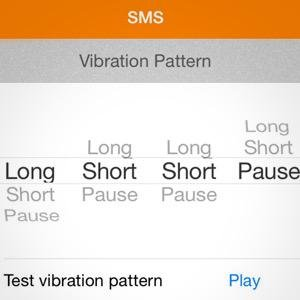
\includegraphics[width=\textwidth]{pics/martian.jpg}
	\end{minipage}
	\caption{Einstellungsm{\"o}glichkeit auf der Apple Watch (links) und in der Martian App (rechts)}
	\label{fig:Bild10}
\end{figure}

%\begin{figure}
%	\centering
%    
\includegraphics[width=\textwidth]{pics/applewatch.png}
%    \caption{Settings on the apple watch}
%    \label{fig:applewatch}
%\end{figure}
 
%% ==============================
\subsection{iPhone}
%% ==============================
\label{ch:Grundlagen:sec:RelatedWork:subsec:PersonalisierteVibration}

\begin{figure}
	\centering
    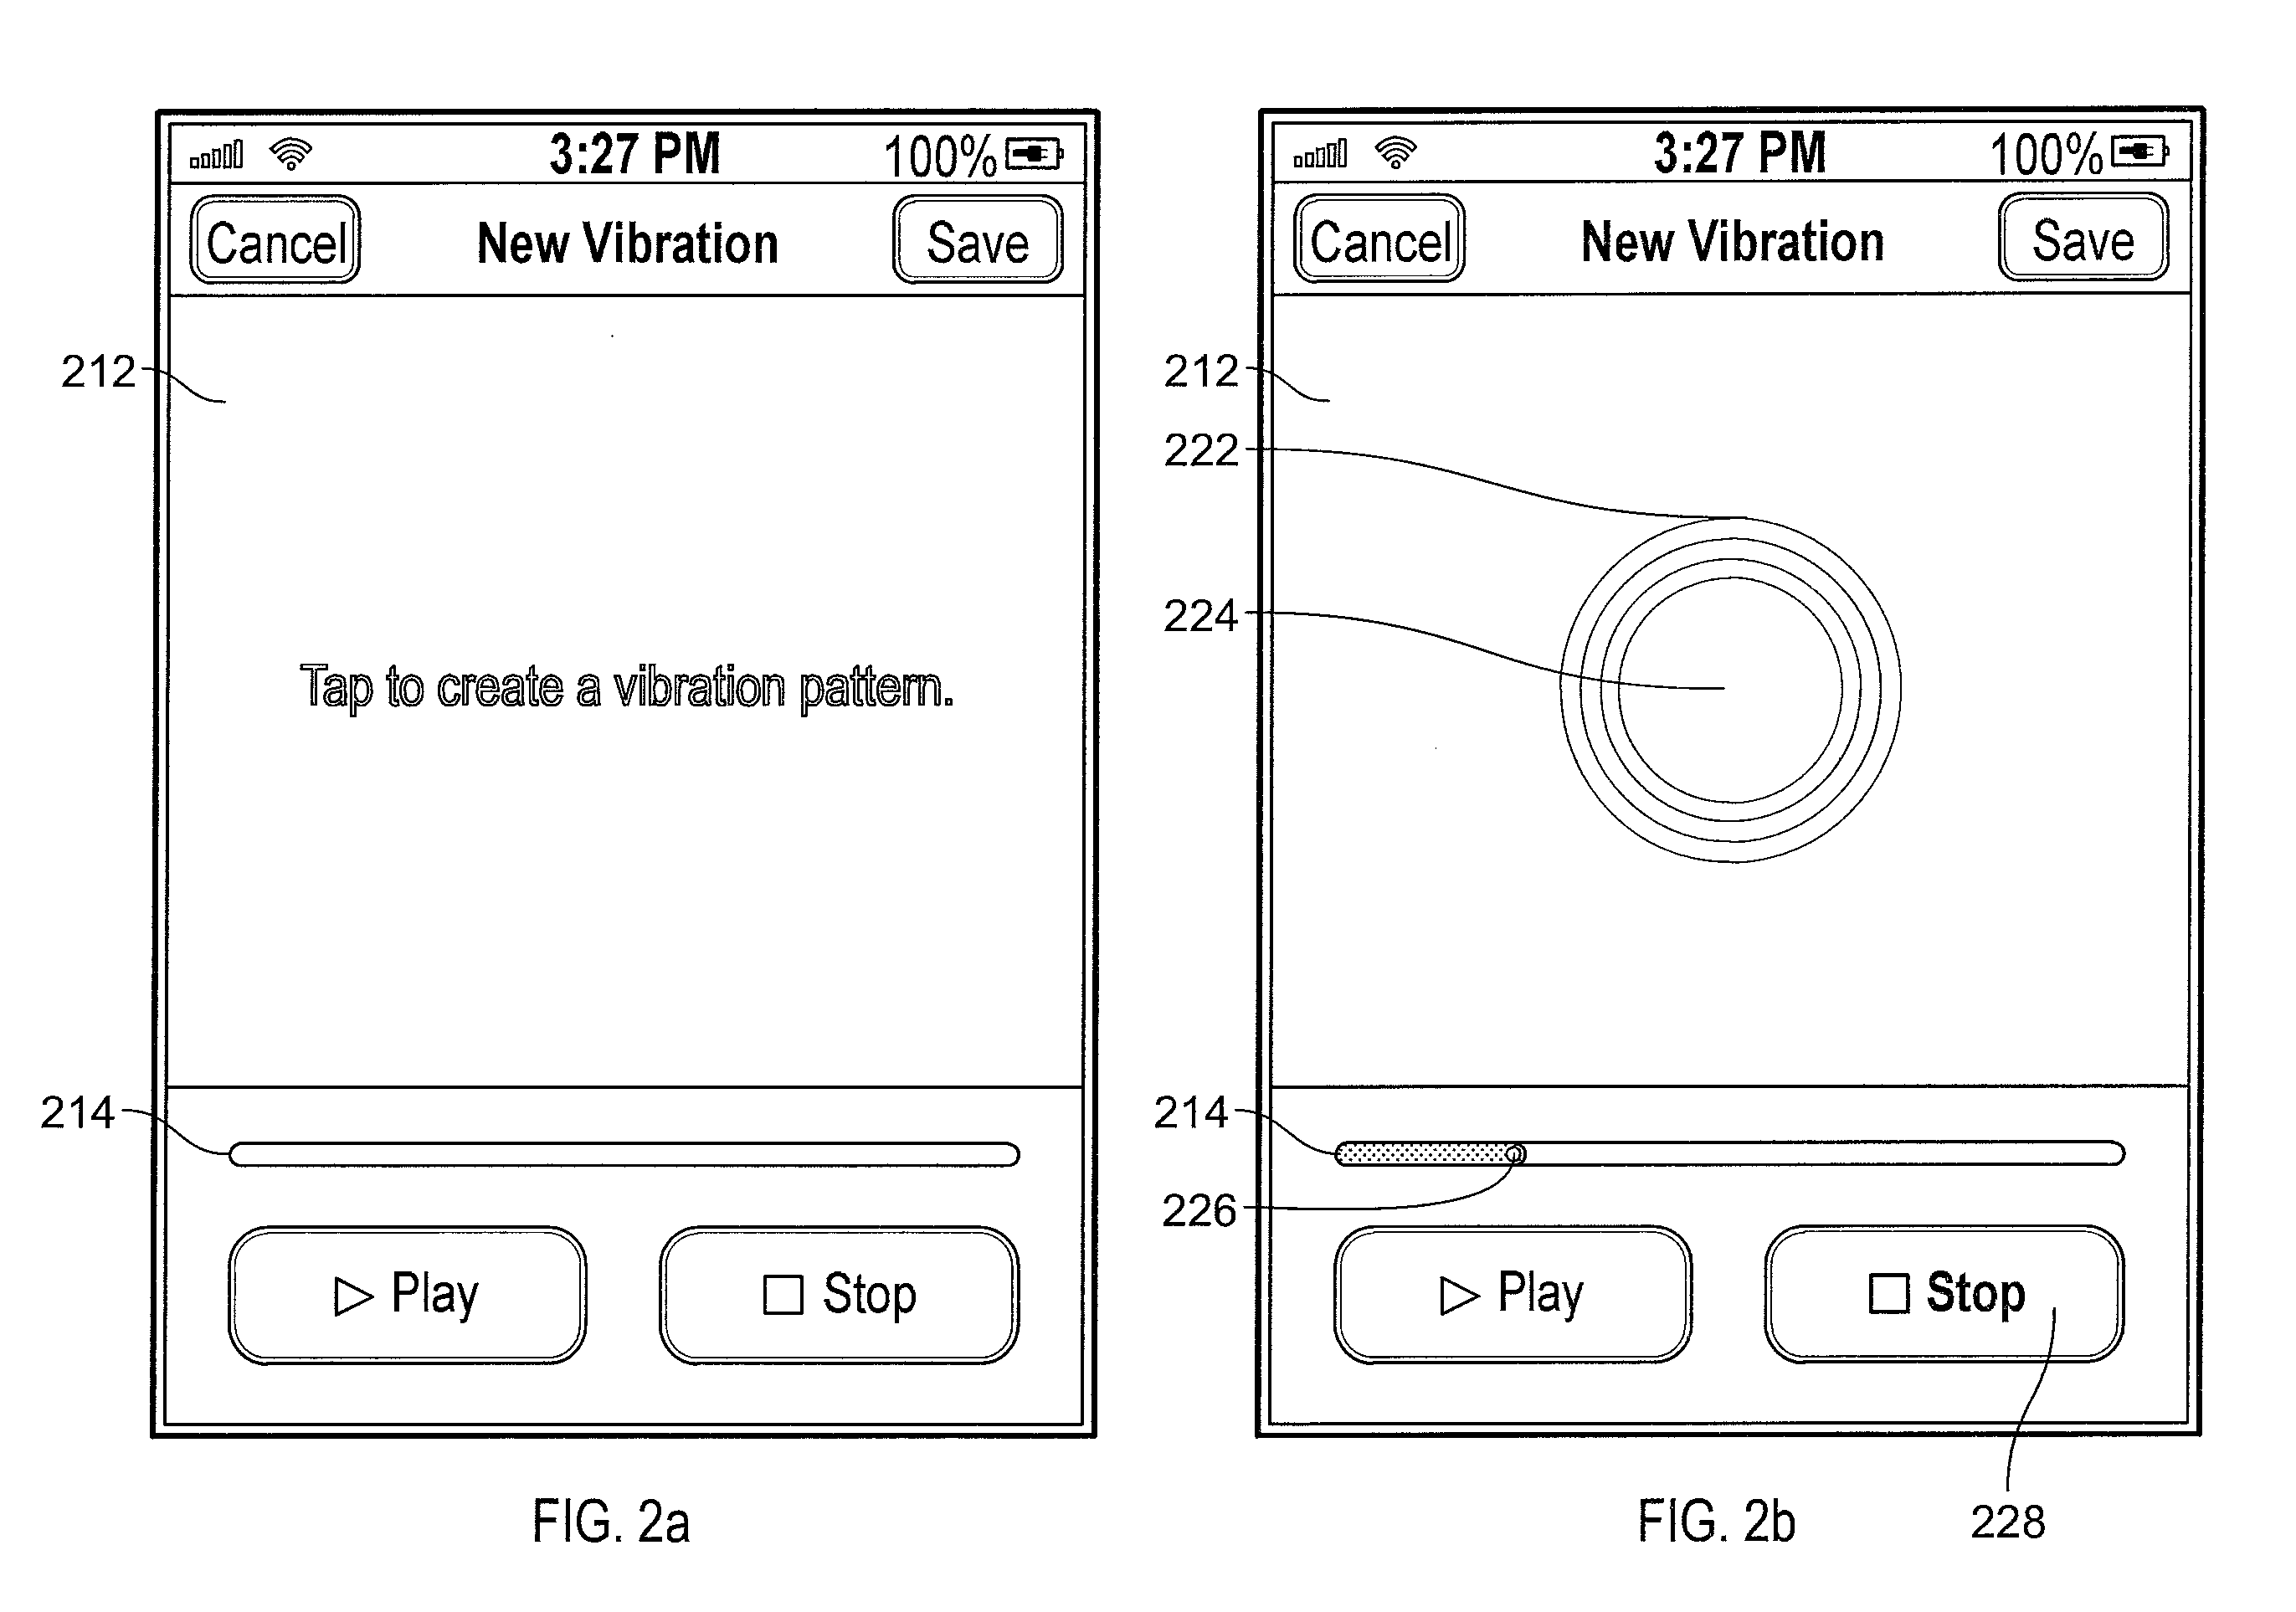
\includegraphics[width=\textwidth]{pics/iphone.png}
    \caption{Erstellung eigener Vibrationsmuster auf dem iPhone}
    \label{fig:iphone}
\end{figure}

Der Hersteller Apple hat auch bei dem iPhone eine M{\"o}glichkeit geboten, eigene Vibrationsmuster zu erstellen, jedoch mit Einschr{\"a}nkungen.
Wenn man in die jeweilige Einstellung der iPhones gelangt, erscheint das folgende Bild \autoref{fig:iphone}. 
Beim Dr{\"u}cken auf das Display wird an der Stelle eine Vibration erzeugt. 
Man hat 10 Sekunden um ein eigenes Muster zu erzeugen, indem man wiederholt auf den Bildschirm dr{\"u}ckt. 
An der Stelle, an der man den Bildschirm ber{\"u}hrt hat, erscheint visuell um der Position ein Kreis. 
Die erzeugten Vibrationen werden in einer Leiste visuell angezeigt. 
Man kann sich beliebig viele Vibrationsmuster speichern, die bis zu 10 Sekunden lang sind. \cite{fleizach2016custom}

Die Einschr{\"a}nkung, die man hier erw{\"a}hnen muss ist, dass man die Vibrationsmuster nur f{\"u}r Systeminterne Funktionen benutzen kann. 
Dies bedeutet, dass man die Funktionen f{\"u}r Klingelt{\"o}ne, Nachrichtent{\"o}ne, Erinnerungshinweise, Kalenderhinweise (o. {\"a}.) hinzuf{\"u}gen kann. 
F{\"u}r eine andere Anwendung, die nicht im Betriebssystem integriert sind, ist das nicht m{\"o}glich. 
Somit k{\"o}nnen Benachrichtigungen von anderen Entwicklern keine eigenen Vibrationsmuster erhalten. 
Tr{\"a}gt man das iPhone in der Hosentasche und es wird eine Benachrichtigung einer Applikation empfangen, die nicht im System integriert ist, kann man anhand der Vibrationen des iPhones nicht unterscheiden, welche Application dies gewesen ist.
%Daraus folgt, wenn das iPhone in der Hosentasche ist und ich eine Benachrichtigung von einer Application erhalte, die nicht im System integriert gewesen ist, kann man anhand der Vibrationen des iPhones nicht unterscheiden welche Application dies gewesen ist.
% kann man bei Benachrichtigungen von anderen Entwicklern nicht anhand der Vibrationen des iPhones  unterscheiden.

%% ==============================
\subsection{Martian Smartwatch}
%% ==============================
\label{ch:Grundlagen:sec:RelatedWork:subsec:PersonalisierteSmartwatch}

%\begin{figure}
%	\centering
%    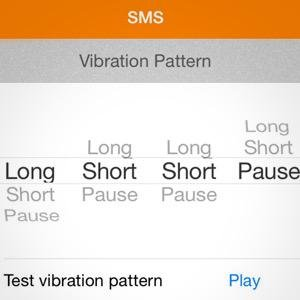
\includegraphics[width=\textwidth]{pics/martian.jpg}
%    \caption{possible settings on the martian watch}
%    \label{fig:martian}
%\end{figure}

Das Ger{\"a}t, das es nach meiner Recherche am besten gel{\"o}st hat, ist eine Smartwatch von einem kleinen Startup namens Martian. 
Das Startup hat eine Uhr hergestellt, mit der man mittels einer App auf dem Smartphone die Vibrationsmuster selbst anpassen kann. 
Die App unterst{\"u}tzt eine gro{\ss}e Anzahl an Applikationen, von anderen Herstellern, die Benachrichtigungen senden. 
Ein Vibrationsmuster f{\"u}r die Uhr kann man aus mit zu 4 Signalen auf der Uhr darstellen. 
Die Signale sind als Lang, Kurz und Pause festgelegt. 
Somit kann man mittels der Vibration der Uhr herausfinden, welche App gerade eine Benachrichtigung auf mein Handy gesendet hat. 
Die L{\"a}nge und St{\"a}rke eines Signals sind vom Hersteller festgelegt und kann nicht ge{\"a}ndert werden.

%% ==============================
\subsection{Andere Hersteller}
%% ==============================
\label{ch:Grundlagen:sec:RelatedWork:subsec:PersonalisierteSmartwatch}
Bei sehr vielen Herstellern ist es aktuell noch gar nicht m{\"o}glich eigene Vibrationsmuster zu erstellen. 
Bei Android Ger{\"a}ten ist es aktuell so, dass man aus einer Menge von wenigen vordefinierten Vibrationsmustern sich nur einen ausw{\"a}hlen kann. 
Einige Entwickler haben dieses Problem erkannt und eigene Applikationen entwickelt, die im Store ver{\"o}ffentlicht sind.









%%% Local Variables: 
%%% mode: latex
%%% TeX-master: "diplarb"
%%% End: 
